
%% Web interface
\section*{The Web Interface}

The purpose of the web interface is to grant a simpler way to users for interacting with the interpreters.
This is split up in two parts:
The server, which handles the routing of the web server and serves the client interface, along with api-calls for the actual interaction with the Command-Line Interpreters;
The client part, which is the actual web interface that the user sees.
The implementation of these are described in the following subsections.

\subsection*{Client Interface}

%%%%%%%%%%%%%%%%%%%
%%% Features
%%%%%%%%%%%%%%%%%%%

\noindent
Before explaining the implementation of the client interface, the features of the interface will be described.
If we look at the User Interface seen in Figure \ref{fig:web_client_ui}, we have 3 rectangular areas: The toolbar at the top; the code editor, located below the toolbar on the left hand side; the result area, located below the toolbar on the right hand side.

\begin{figure}[H]
  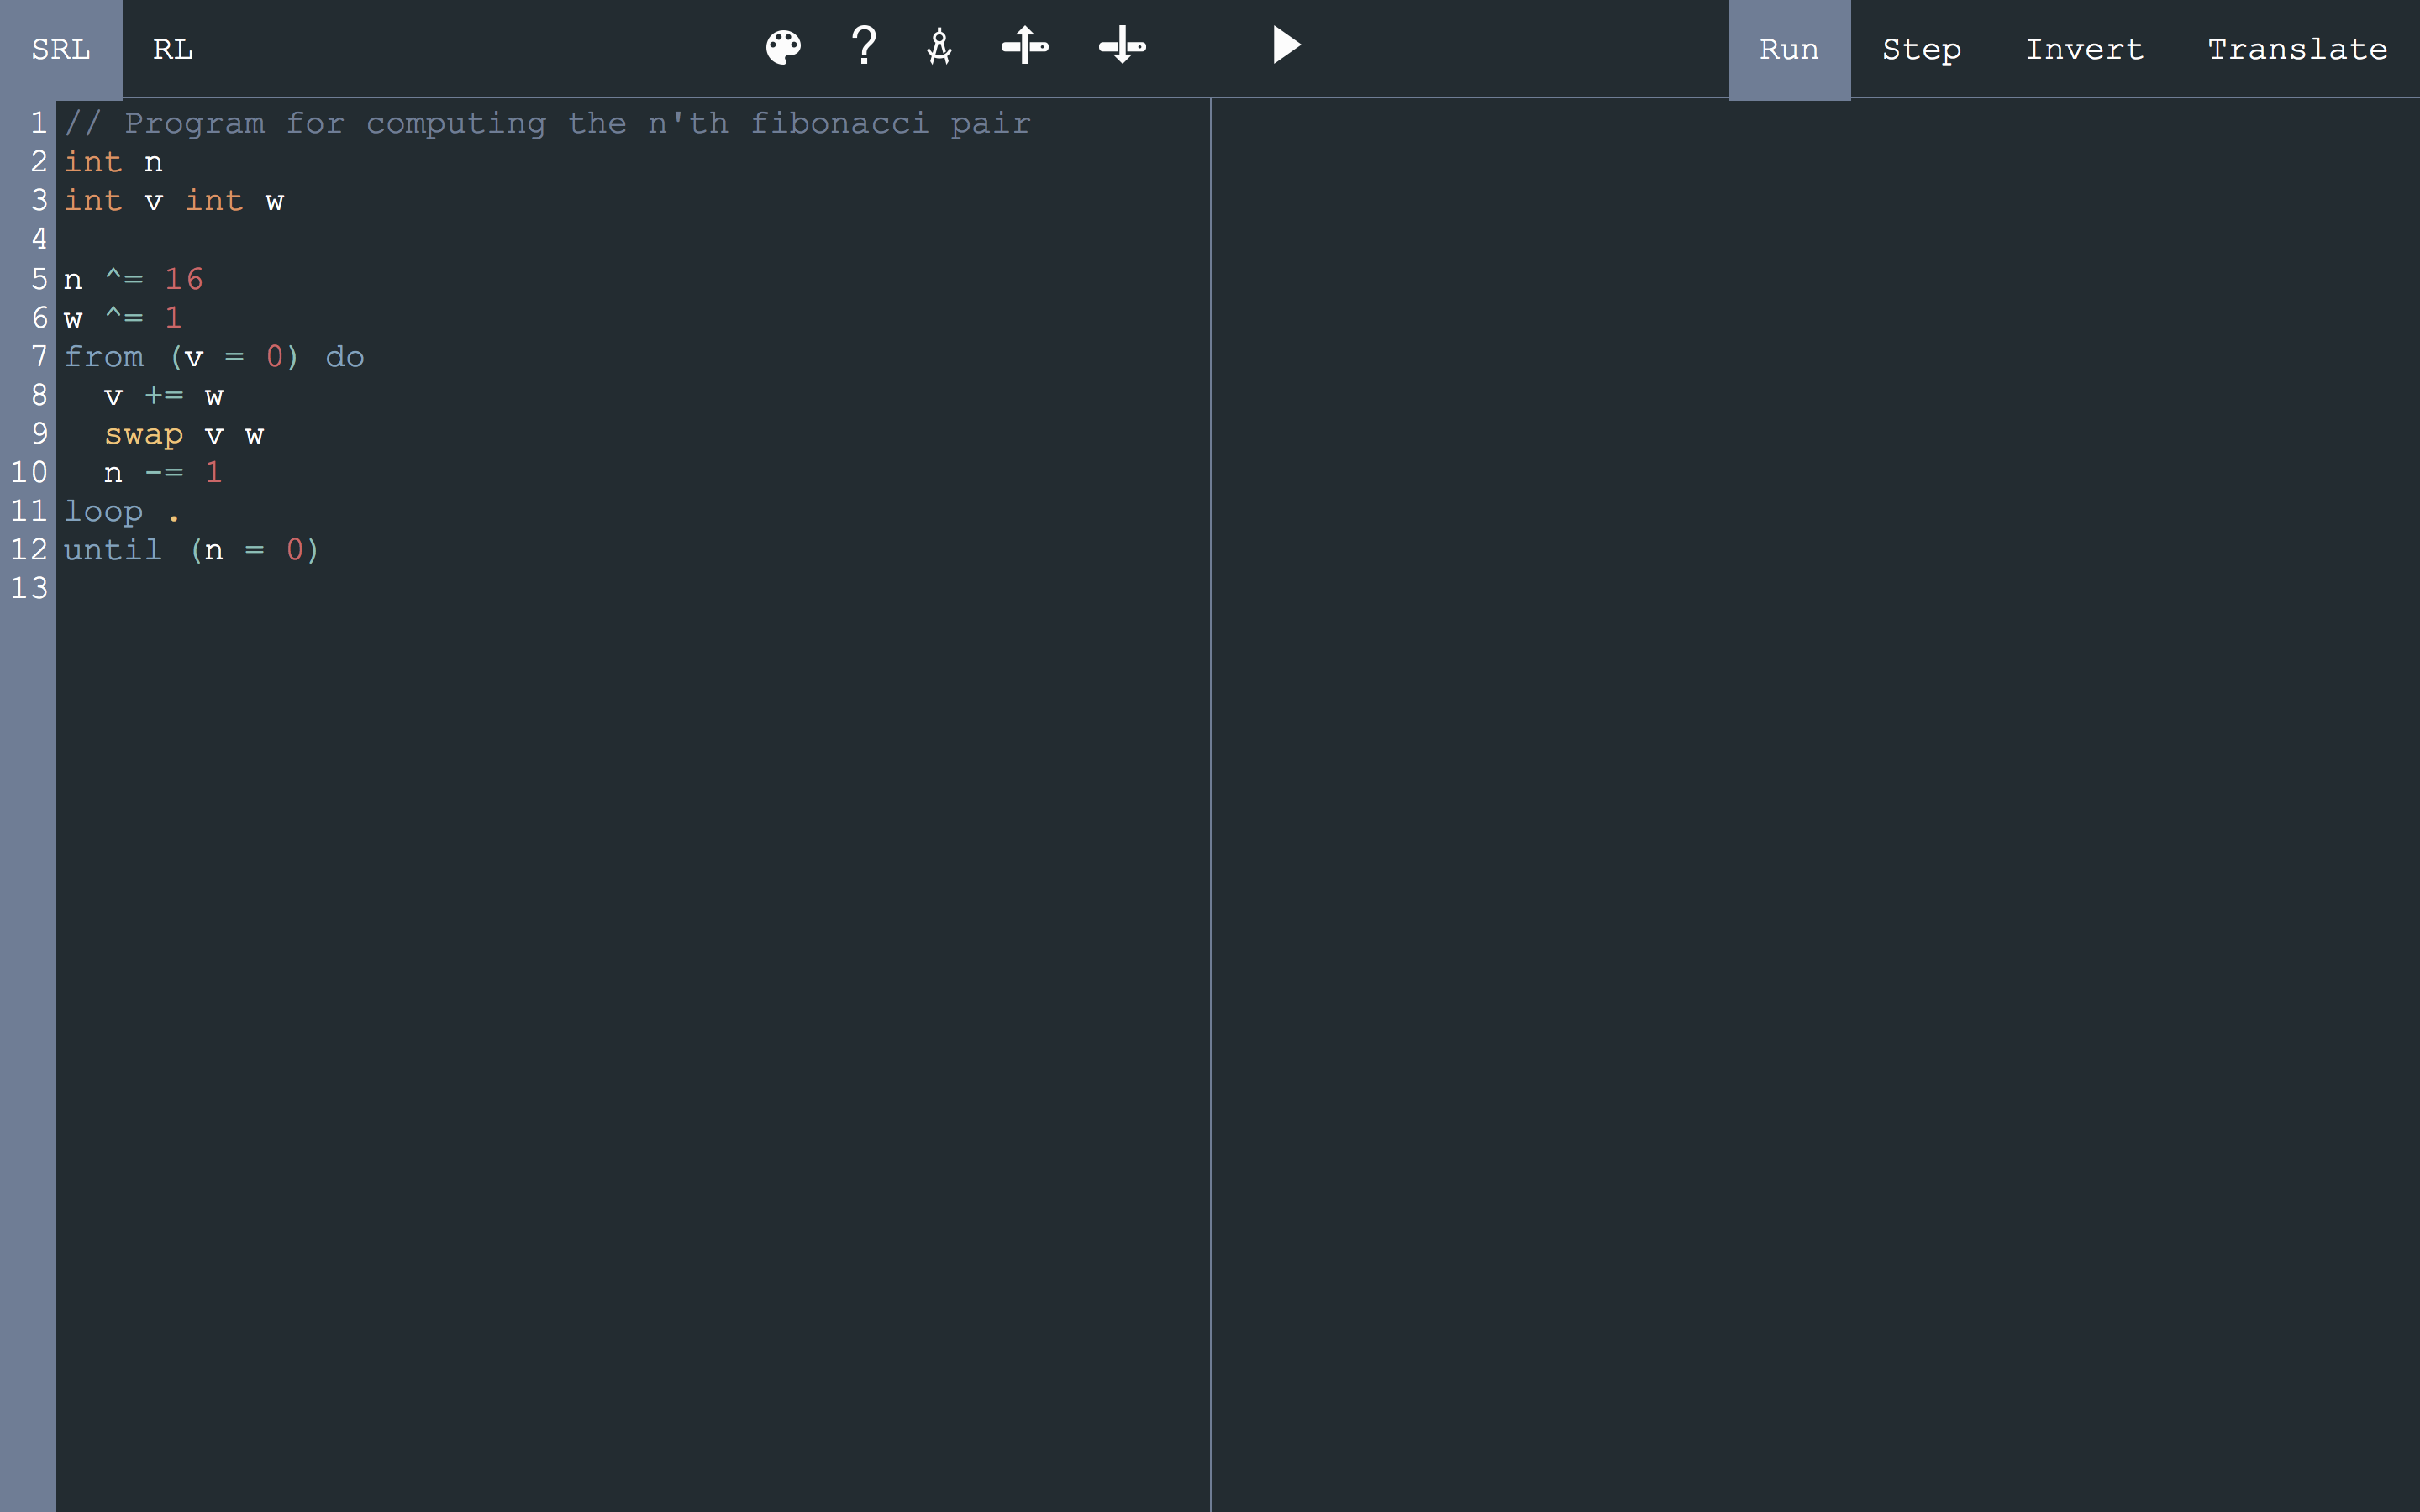
\includegraphics[width=\textwidth]{web_client_ui.png}
  \caption{Screenshot of web client UI.}
  \label{fig:web_client_ui}
\end{figure}

\noindent
At the far left of the toolbar a radio button group with the options SRL and RL. The highlighted option indicates how the code in the code editor should be interpreted. If RL is chosen, the code is interpreted as if it were a RL program; likewise for SRL.\\
On the left hand side of the middle, the toolbar has some icons:\\

\begin{description}

  \item[\inlineicon{themes.png} Themes]~\\
    By hovering over the icon a dropdown menu, for choosing the color scheme/ theme of the client interface, appears as illustrated in Figure \ref{fig:web_client_themes}.\\
    Figure \ref{fig:web_client_white_ui} shows the color scheme when the white theme is chosen.\\
    \begin{figure}[H]
      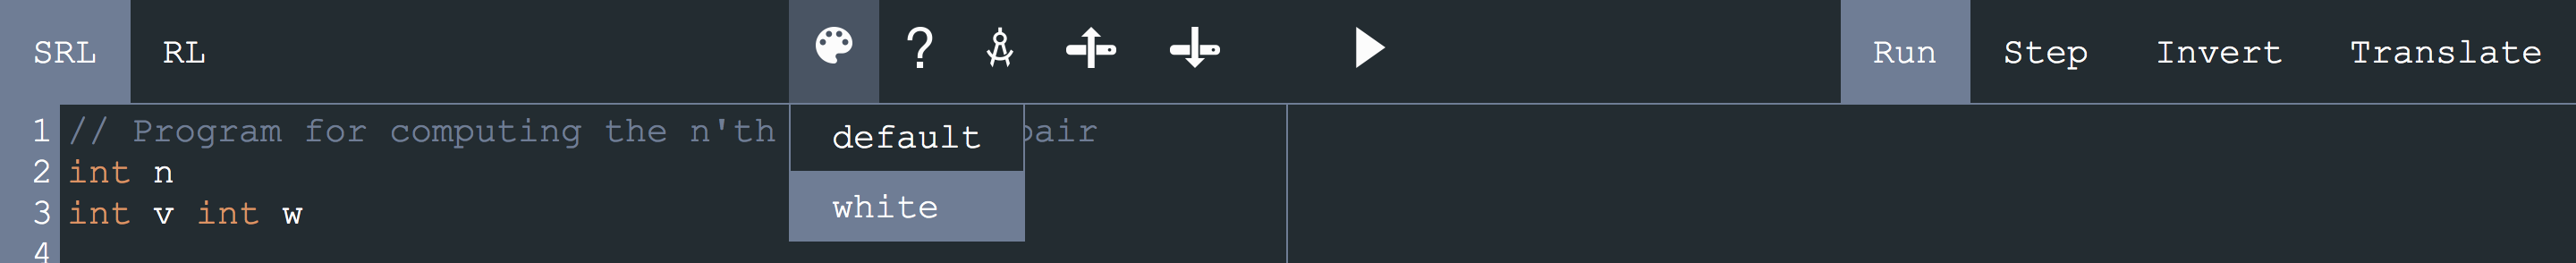
\includegraphics[width=\textwidth]{web_client_themes.png}
      \caption{Web client themes dropdown menu.}
      \label{fig:web_client_themes}
    \end{figure}
    \begin{figure}[H]
      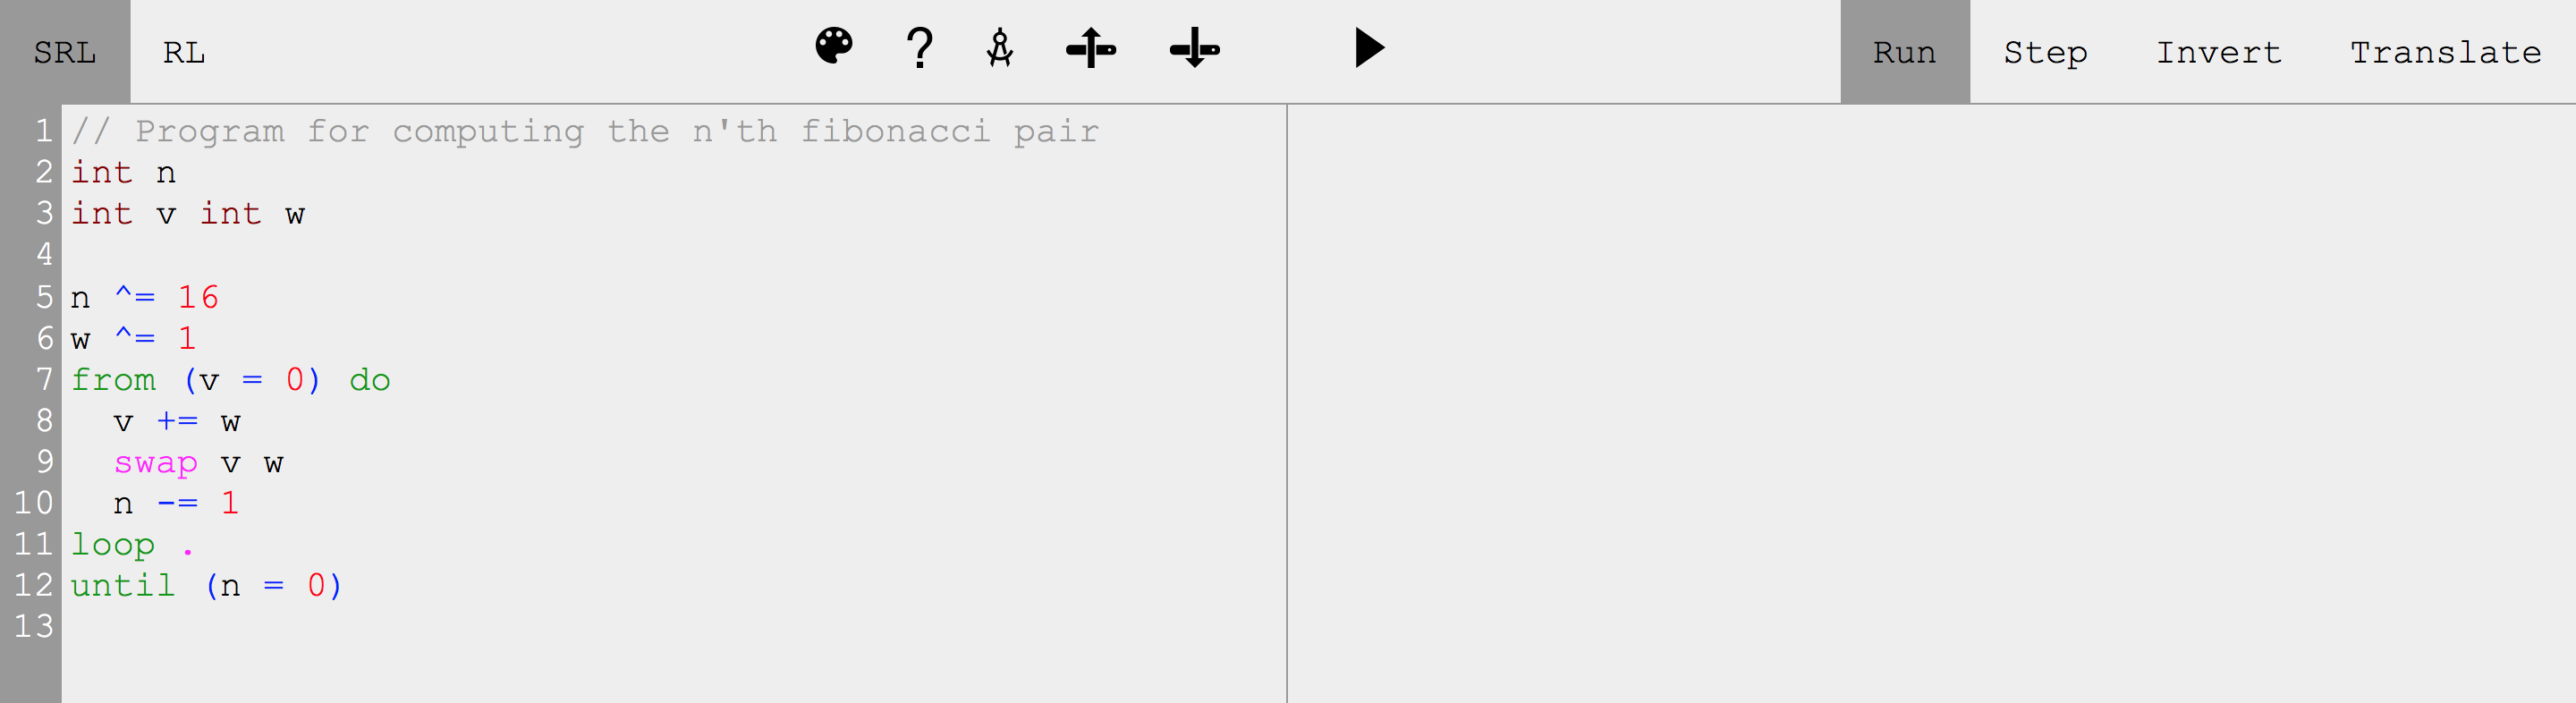
\includegraphics[width=\textwidth]{web_client_white_ui.png}
      \caption{Web client UI in white theme color scheme.}
      \label{fig:web_client_white_ui}
    \end{figure}

  \item[\inlineicon{help.png} Help]~\\
    By clicking on this icon a modal window opens, illustrated in Figure \ref{fig:web_client_help}, with help for the web interface, the modes and the languages.\\
    \begin{figure}[H]
      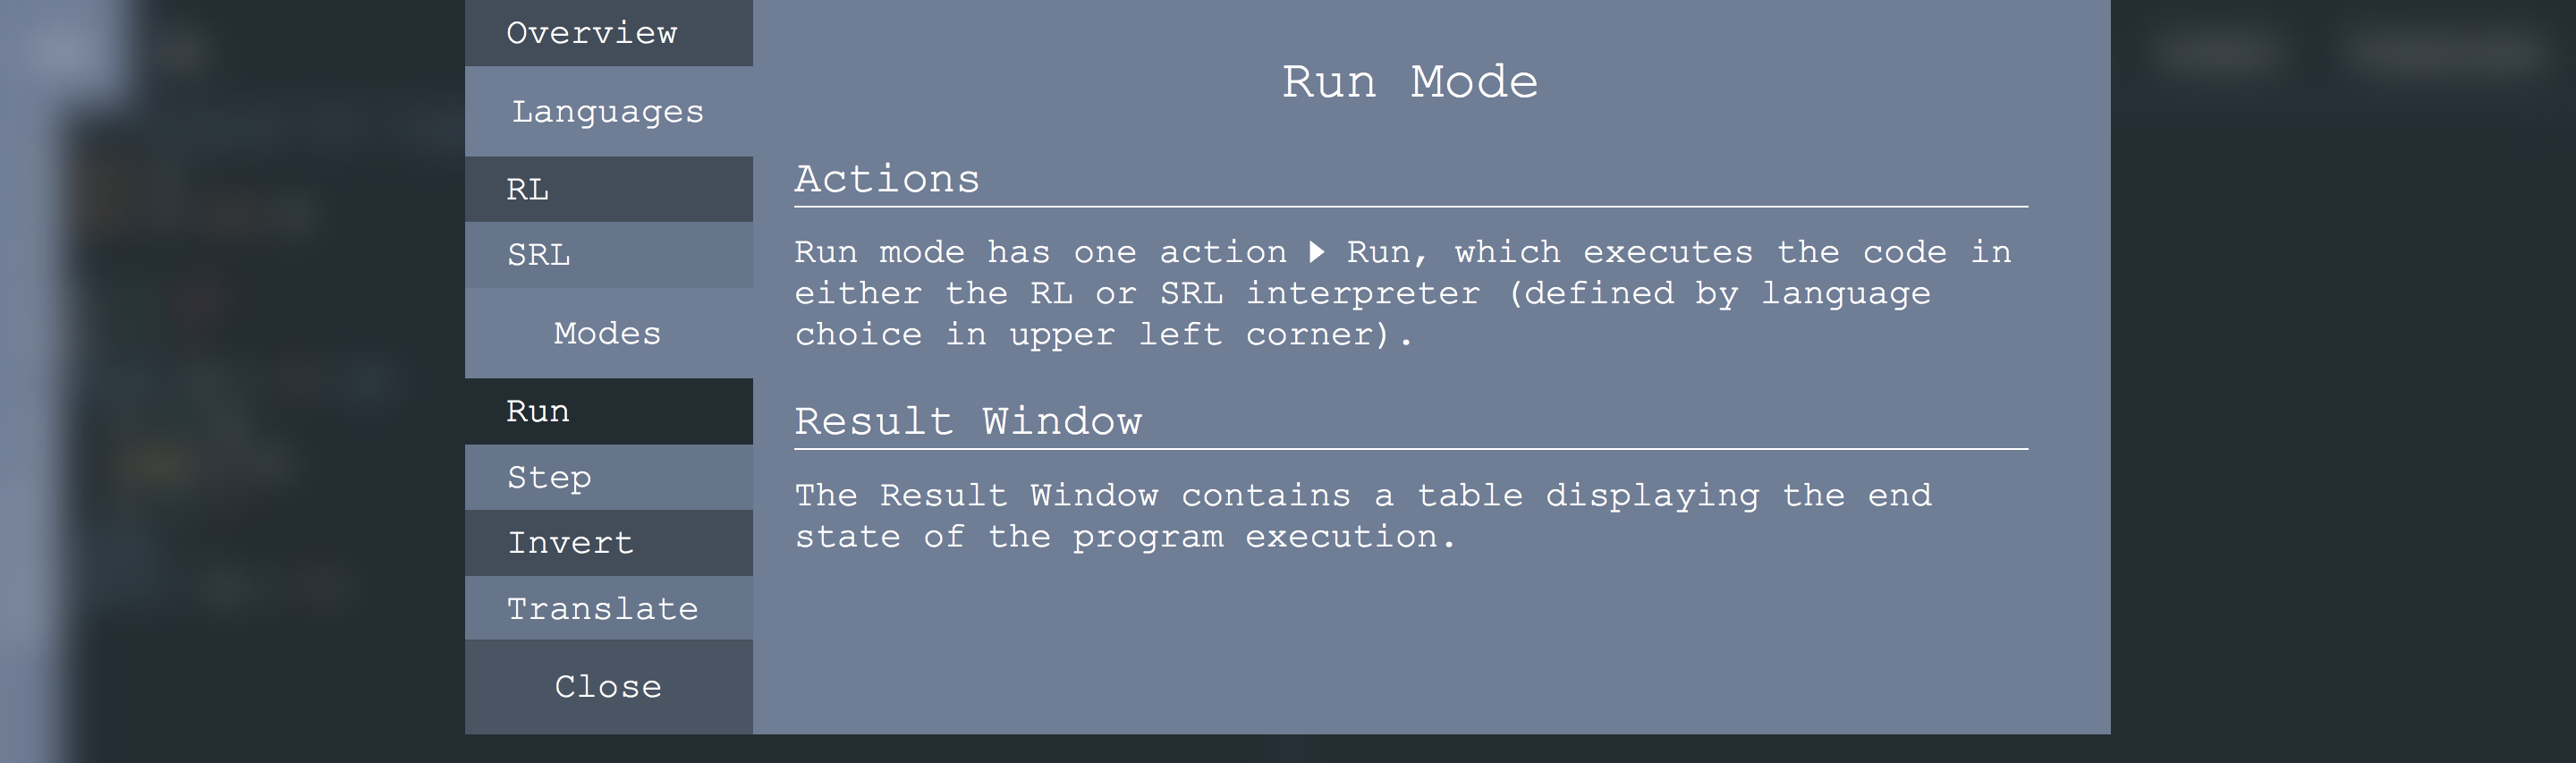
\includegraphics[width=\textwidth]{web_client_help.png}
      \caption{Web client help modal window displaying the Run mode help page.}
      \label{fig:web_client_help}
    \end{figure}

  \item[\inlineicon{template.png} Templates]~\\
    By hovering over this icon a dropdown menu, where template programs for both RL and SRL can be loaded into the code editor, appears as illustrated in Figure \ref{fig:web_client_templates}.\\
    \begin{figure}[H]
      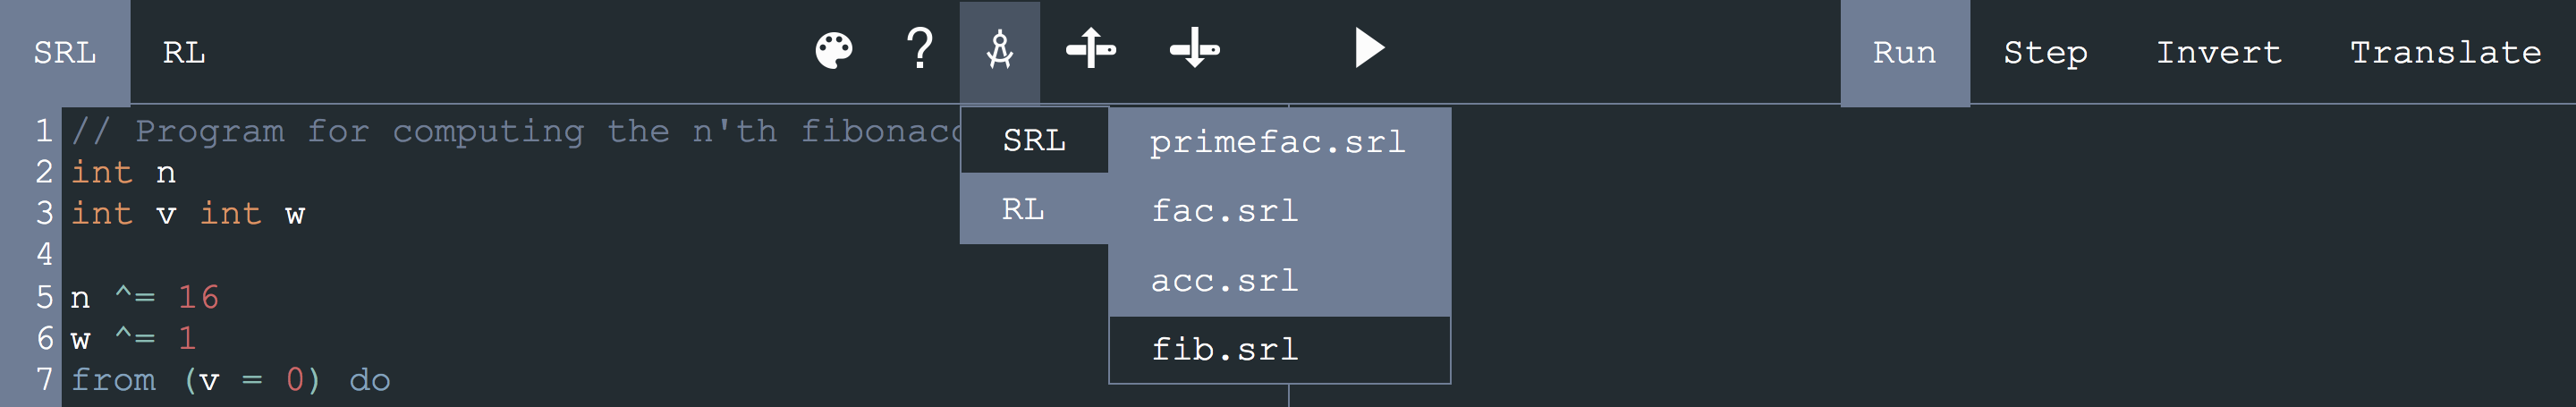
\includegraphics[width=\textwidth]{web_client_templates.png}
      \caption{Web client templates dropdown menu.}
      \label{fig:web_client_templates}
    \end{figure}

  \item[\inlineicon{open.png} Open]~\\
    By click on this icon a modal window opens, as illustrated in Figure \ref{fig:web_client_open}. Here it is possible to import and open previously stored programs.\\
    \begin{figure}[H]
      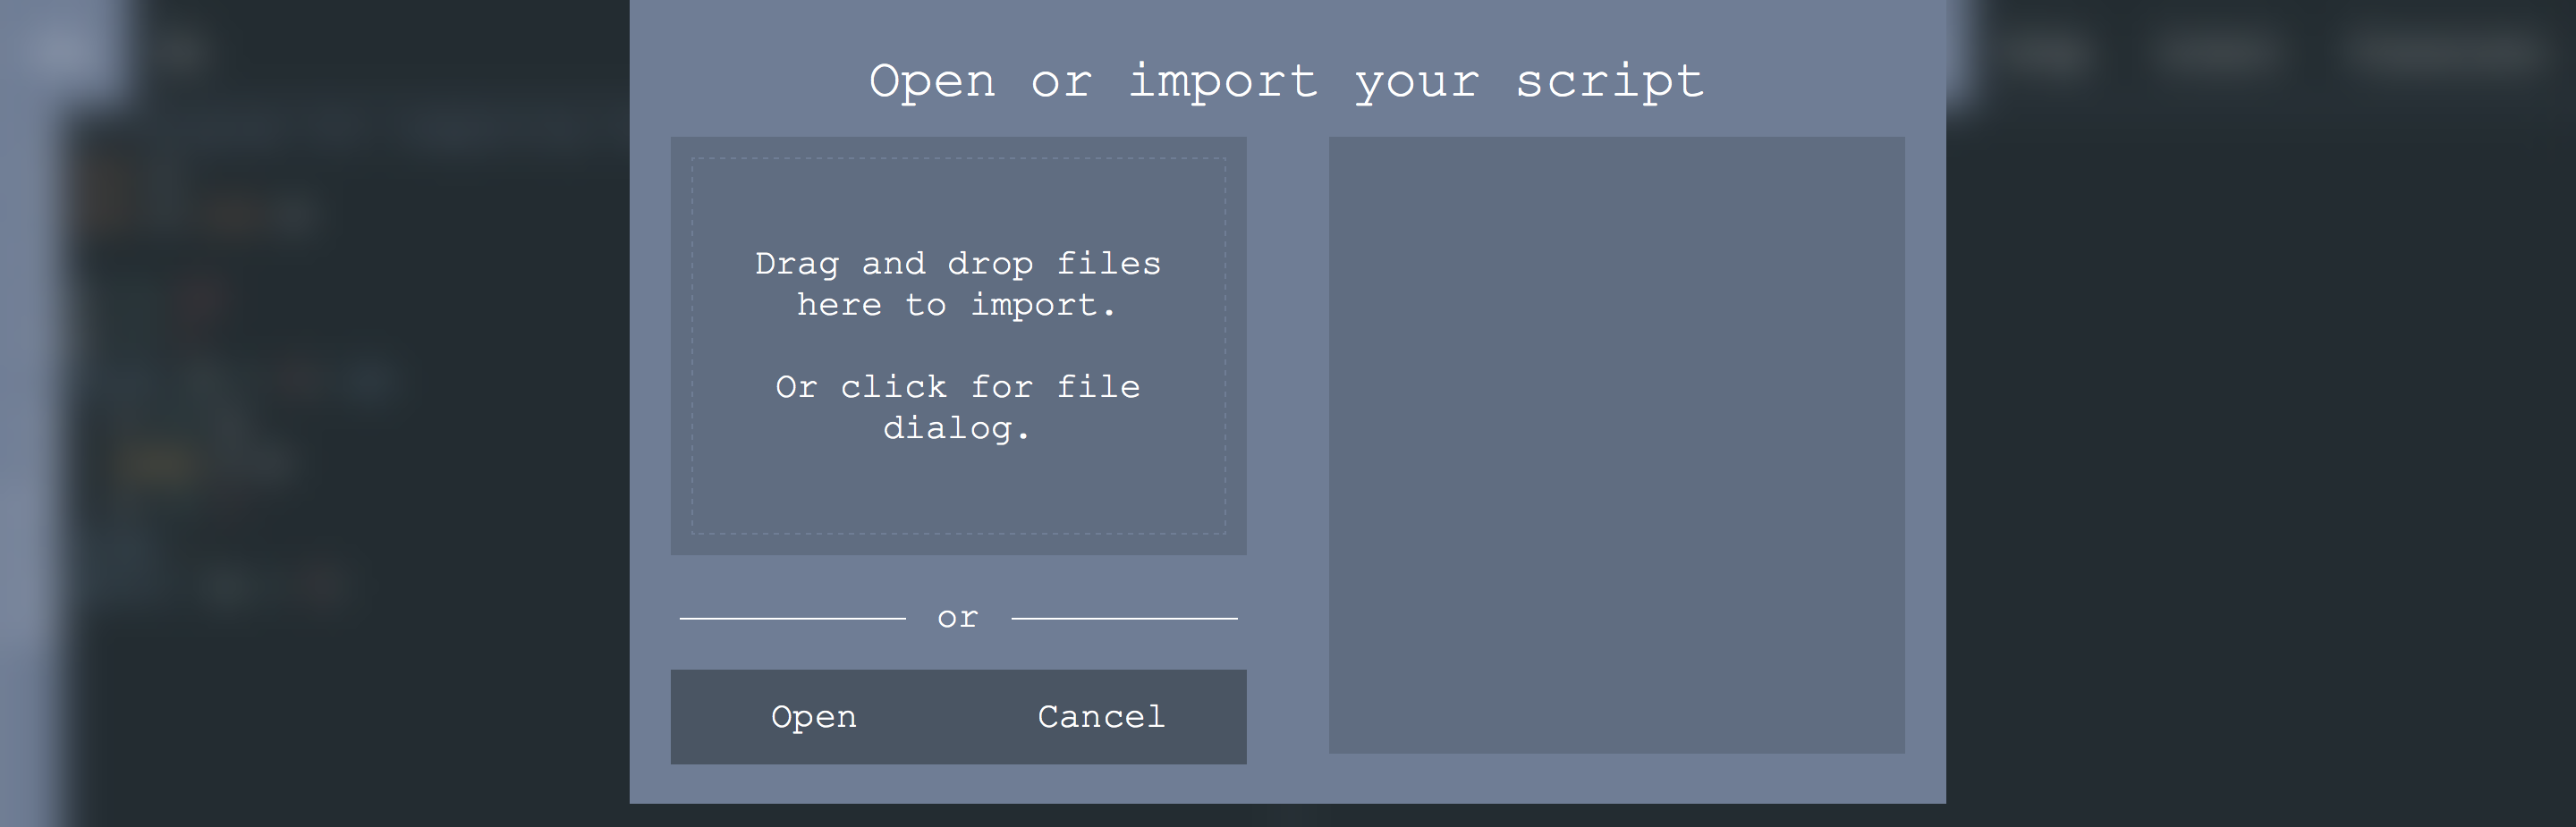
\includegraphics[width=\textwidth]{web_client_open.png}
      \caption{Web client open modal window.}
      \label{fig:web_client_open}
    \end{figure}

  \item[\inlineicon{save.png} Save]~\\
    By clicking on this icon a modal window opens, as illustrated in Figure \ref{fig:web_client_save}. Here it is possible to export, share and store the code currently loaded into the code editor.\\
    \begin{figure}[H]
      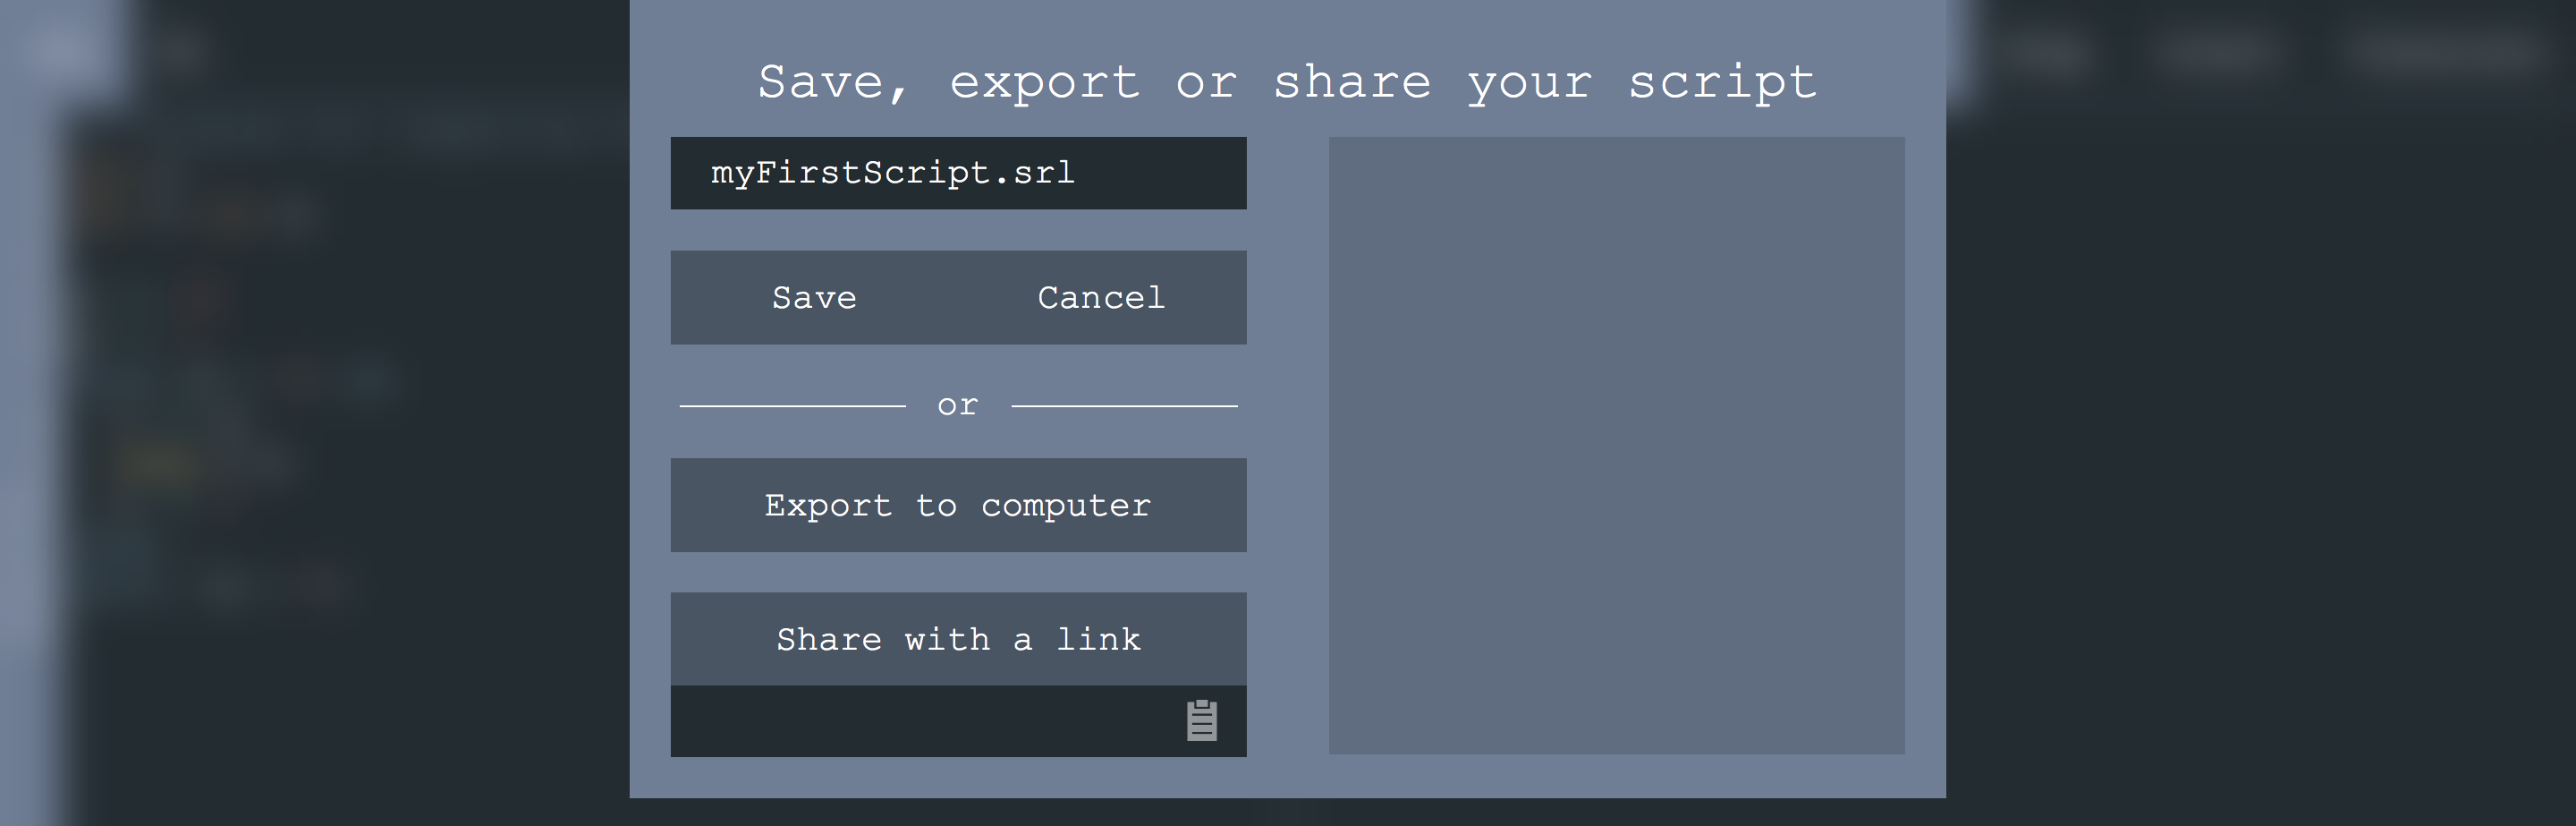
\includegraphics[width=\textwidth]{web_client_save.png}
      \caption{Web client save modal window.}
      \label{fig:web_client_save}
    \end{figure}

\end{description}

\noindent
The right hand side of the toolbar is dedicated to modes and their associated actions. There are 4 modes which are selected from the radio button group at the far right:\\

\begin{description}

  \item[Run]~\\
    The Run mode utilises the run mode from the Command-Line Interface. The only action associated with the Run mode is \inlineicon{play} \textbf{run}, which executes the code written in the code editor, and displays the final program-state in the result area.\\

  \item[Step]~\\
    The Step mode utilises the run mode as the Run mode, but sets the \-\-log flag, to get the execution log instead of only the final state. This way, it is easy to step through the program step by step operation, and see how the individual statements alters the state.
    The execution of the last step operation can either result in successful or erroneous program termination.
    When choosing the Step mode, it is not yet activated.
    For activating the mode, the action \inlineicon{play} \textbf{begin stepping} is used.
    This displays either an error or the start state of the program (all variables set to empty).
    When activated 5 actions are available:
    \inlineicon{prev} \textbf{previous step} undoes the last executed step operation;
    \inlineicon{next} \textbf{next step} executes the next step operation;
    \inlineicon{reset} \textbf{reset} undoes all executed step operations;
    \inlineicon{exec} \textbf{end} executes all remaining step operations;
    \inlineicon{stop} \textbf{stop} stops the execution and deactivates the Step mode.\\
    While Step mode is activated, all other features are disabled.\\

  \item[Invert]~\\
    The Invert mode utilises the invert mode from the Command-Line Interface. The only action associated with the Invert mode is \inlineicon{play} \textbf{invert}, which inverts the code and displays it in the result area.\\

  \item[Translate]~\\
    The Translate mode utilises the translate mode from the Command-Line Interface.
    The only action associated with the Translate mode is \inlineicon{play} \textbf{translate}, which translates the code and displays it in the result area.\\

\end{description}

\noindent
All the above modes have the ability to fail. Figure \ref{fig:web_client_error} illustrates a case where a parse error occurs.

\begin{figure}[H]
  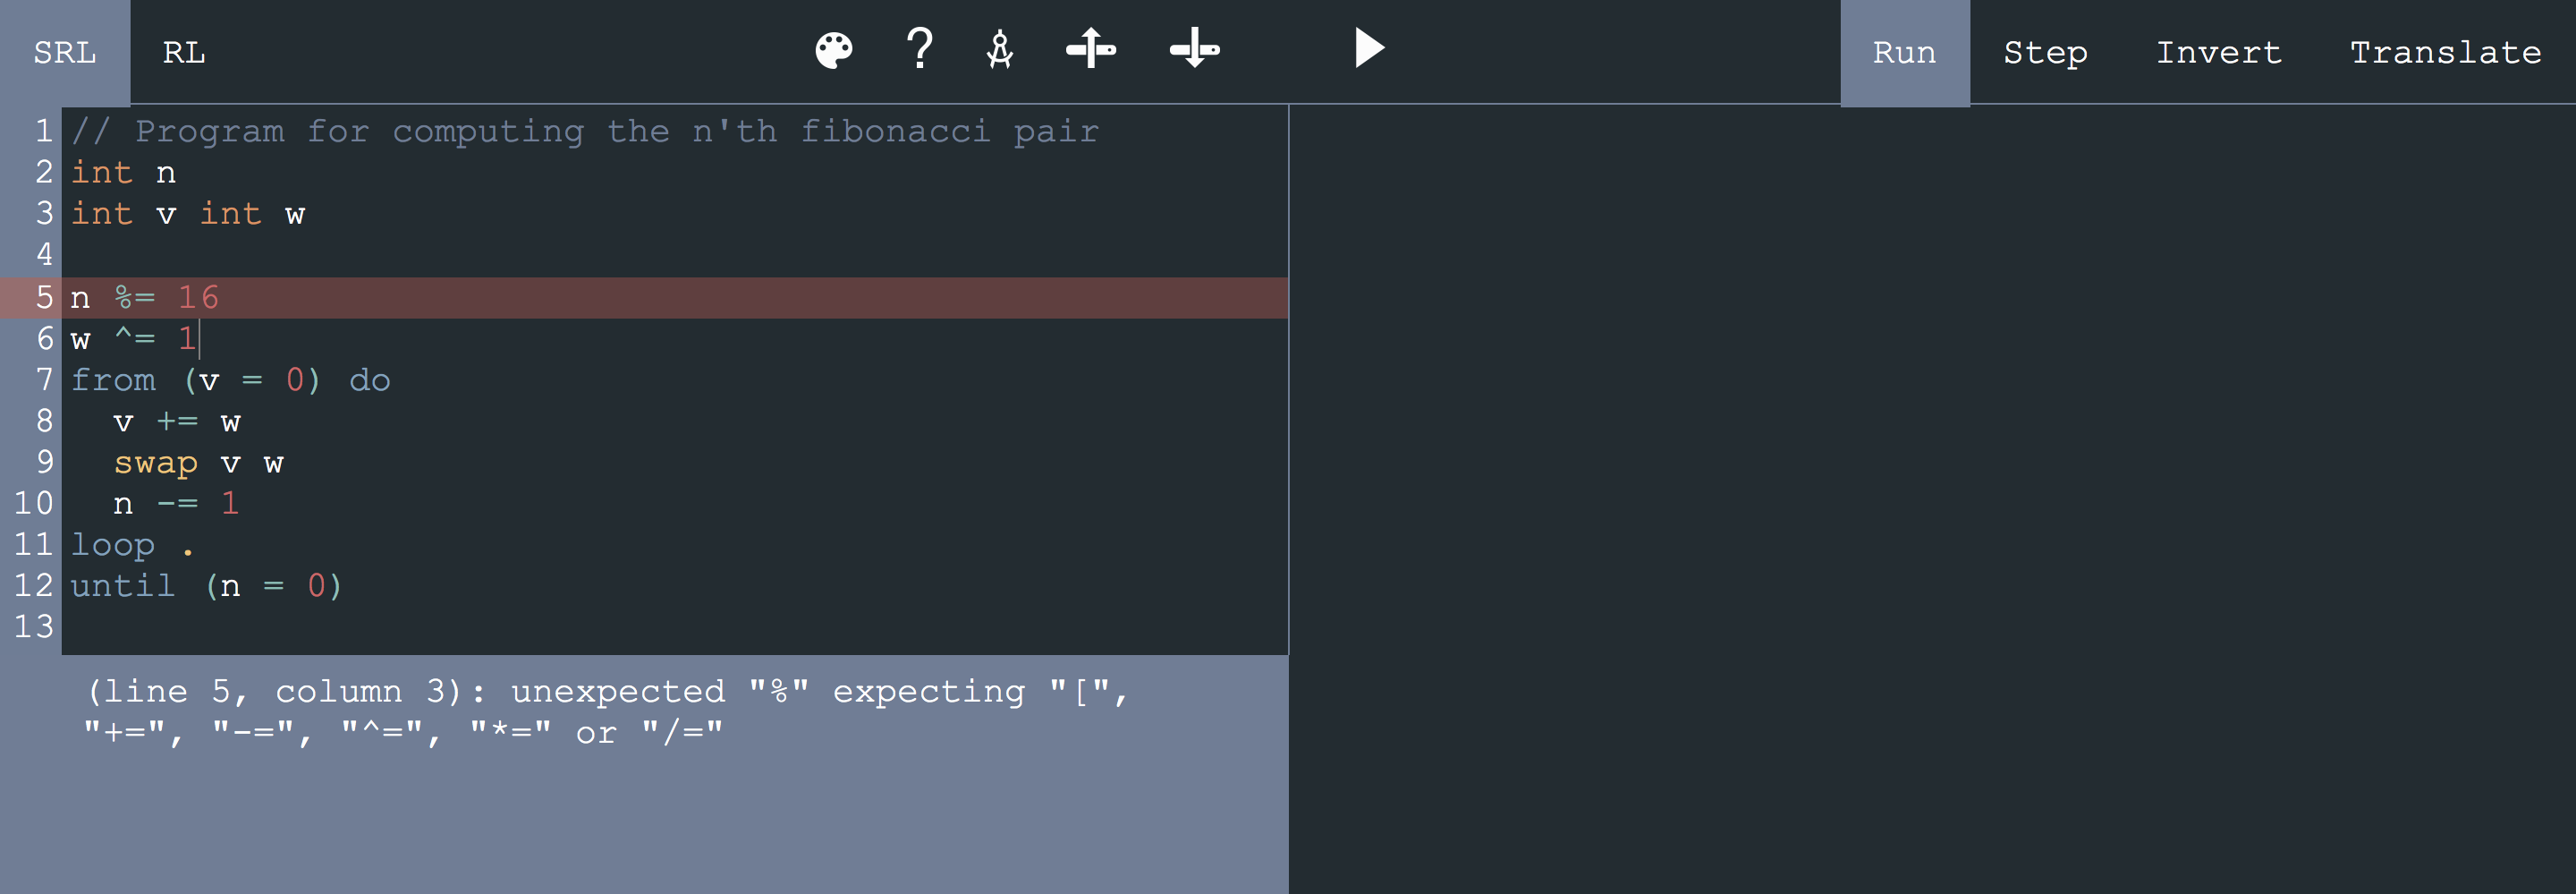
\includegraphics[width=\textwidth]{web_client_error.png}
  \caption{Web client with parse error.}
  \label{fig:web_client_error}
\end{figure}

%%%%%%%%%%%%%%%%%%%
%%% Implementation
%%%%%%%%%%%%%%%%%%%

\noindent
Now that the features has been introduced, we can look at the implementation hereof.
The web client interface is a nodeJS project written in ECMAScript 6, using the library ReactJS, for creating modularised components.
We chose to use ReactJS, instead of vanilla javascript and html, since it allows component rendering based on state.
This way focus was primarily on state and logic, instead of design and propagating state to the application.
To separate state and logic from UI even further, we chose to handle state through Redux.
This way we could move state and alteration to state outside of the ReactJS components. Hereby giving the individual components access to only the absolute necessary state variables, and state alterations methods.
This way the possibilities where a specific state alteration can fail is limited to the components with access, and hereby making it easier to debug and fix.\\

\noindent
The web client interface uses babel and webpack to compile and bundle scripts and resources.
Webpack uses babel to convert JSX to React components and transpile ECMAScript 6 to ECMAScript 5, to allow for \texttt{import} statements.
Webpack itself is used to precompile SASS, which is used for styling, to CSS, appending prefixes to the CSS for better cross-browser support and bundling scripts, styles and assets for minimal HTTP requests.\\

\noindent
The root of the web client is \path{/web/client}. Configuration files for node package dependencies and the webpack build flow are found here.
Under the subdirectory \path{src/} are all source files and resources located.
ReactJS components are found under \path{src/components} and the corresponding styling/ SASS files are found under \path{src/styles} along with the theme color schemes in the subdirectory \path{src/styles/themes}.\\

\todo{App component}
\todo{Header component}
  \todo{Radio, Button, Dropdown component}
\todo{Editor component}
  \todo{CodeMirror}
\todo{Result component}
\todo{Modals}
  \todo{HelpModal}
  \todo{OpenModal}
  \todo{SaveModal}




\subsection*{Server \& API}

The web server is an independent node project, when built uses the Client Web Interface and the Command-Line Interface as dependencies.
These are build and copied into the web server project folder.
The executables for the Command-Line Interfaces are placed under \path{/web/server/bin} and the Web Client Interface is placed under \path{/web/server/client}.\\

\noindent
The server is written in ECMAScript 6, but since nodeJS (version 9 and below) does not support \texttt{import} statements natively, the Babel transpiler is used for running the ECMAScript 6 code as ECMAScript 5.
This is done in the entry-file \path{babel-server.js}, as a wrapper for the actual server configuration in \path{server.js}.
We run the transpiled code with node, and uses the Express package for opening ports, setting up the server and handling web-routes.
All communication between the API server and the client-side, is formatted as JSON; as is the results from the interpreters.
This way it is easy to parse data from the interpreter to the client interface via the API.

The server has Cross Origin Resource Sharing (CORS) enabled, to allow for separation of the api server and the client web interface.
This allows for the server to be hosted at one address, while the interface is hosted at another.
CORS is enabled by setting the appropriate headers shown in Listing \ref{lst:cors_setup}.

\lstinputlisting[language=javascript,caption={CORS headers from /web/server/server.js.},label={lst:cors_setup},firstline=10,firstnumber=10,lastline=15]{../web/server/server.js}

The routing has two responsibilities: To handle API calls, which can be seen in Figure \ref{fig:full_api}; serve static files, when the client interface is requested. The defined routes are listed in Figure \ref{fig:server_routes}. Routes are divided into 3 categories: API routes, root requests and static files; where static files are the bundled css and javascript files, that the client interface requires.\\

\begin{figure}[H]
  \begin{tabular}{|l|p{8.7cm}|}\hline
    \textbf{Route} & \textbf{Responsibility}\\\hline
    \texttt{/}     & Fetch the built client interface index page from (\path{/web/server/client/index.html}).\\\hline
    \texttt{/api*} & Here \texttt{*} is everything after \texttt{/api}, which is forwarded to the API router. The API routes are described in Figure \ref{fig:full_api}. \\\hline
    \texttt{/:filename.:ext}     & Here \texttt{:filename.:ext} matches a static resource, e.g. \texttt{bundle.js}. All static files are fetched from \path{/web/server/client}. Thus only files that the client interface uses can be requested.\\\hline
  \end{tabular}
  \caption{Routes for web server.}
  \label{fig:server_routes}
\end{figure}

If the client interface is hosted at a different address than the api, the \path{/web/server/client} folder can be removed, causing the route for the index page and the static pages to respond with a 404 (page not found) status and page.\\

\todo{API - features}\\

\begin{figure}[H]
  \begin{tabular}{|l|l|p{6.7cm}|}\hline
    \textbf{Route} & \textbf{Method} & \textbf{Responsibility}\\\hline
    \texttt{/run/:language} & \texttt{POST} & Here \texttt{:language} can either be \texttt{rl} or \texttt{srl}.
                                                This API-call executes the code that is posted along with the request, and returns the end-state of the program.
                                                The code submitted should be wrapped in a JSON object, with the attribute \texttt{code}.\\\hline
    \texttt{/run/log/:language} & \texttt{POST} & Is equivalent to \texttt{/run/:language}, but instead of returning the end-state
                                                    alone, it also returns the json-formatted execution-log.\\\hline
    \texttt{/invert/:language} & \texttt{POST} & Here \texttt{:language} can either be \texttt{rl} or \texttt{srl}.
                                                This API-call inverts the code.
                                                The code submitted should be wrapped in a JSON object, with the attribute \texttt{code}.\\\hline
    \texttt{/translate/:language} & \texttt{POST} & Here \texttt{:language} can either be \texttt{rl} or \texttt{srl}.
                                                This API-call translates the code from the specified language to its counterpart.
                                                The code submitted should be wrapped in a JSON object, with the attribute \texttt{code}.\\\hline
    \texttt{/template/list}  & \texttt{GET} & Returns a list of SRL and RL files, as a JSON-object. The object has the attributes \texttt{srl} and \texttt{rl}, where each corresponding value is a list of template-names for that language. \\\hline
    \texttt{/template/:file} & \texttt{GET} & Here \texttt{:file} is the template requested.
                                              A JSON-object, with the attribute \texttt{code}, which contains the code of the requested template file, is returned.\\\hline
  \end{tabular}
  \caption{API routes.}
  \label{fig:full_api}
\end{figure}

\todo{Security}
For accessing the Command-Line interface, listing and fetching template-files, the interface execFile(file, [arguments], callback) from the node module

% To secure the application, and the hosting system, most input parameters are validated before the shell commands are executed; the input code is one of the parameters which is not validated.
% To avoid command injections via code input, the execFile interface from nodes child\_process module, is used.
% execFile does not by default open a new shell, but spawns the specified command/ file directly, which minimizes the overhead.
% The

\begin{lstlisting}[language=javascript]
execFile(cmd,
        [mode, code, flags],
        {maxBuffer, timeout},
        (err, stdout, stderr) => {
  // ... callback content
});
\end{lstlisting}
